\section{Solution}

\subsection{Infrastructure}
\subsubsection*{CAVE topologies}
\begin{frame}\frametitle{Infrastructure - CAVE topologies}
	\begin{itemize}
		\item<1-> One-node setup
		\begin{itemize}
			\item 1 node
			\item 4 graphics cards
			\item 8 GB memory
		\end{itemize}
		\item<2-> Six-node setup
		\begin{itemize}
			\item 6 nodes
			\item 1 graphics card per node
			\item 2 GB memory per node
		\end{itemize}
	\end{itemize}
\end{frame}

\subsubsection*{One-node setup}
\begin{frame}\frametitle{One-node setup}
	\begin{figure}
		\centering
	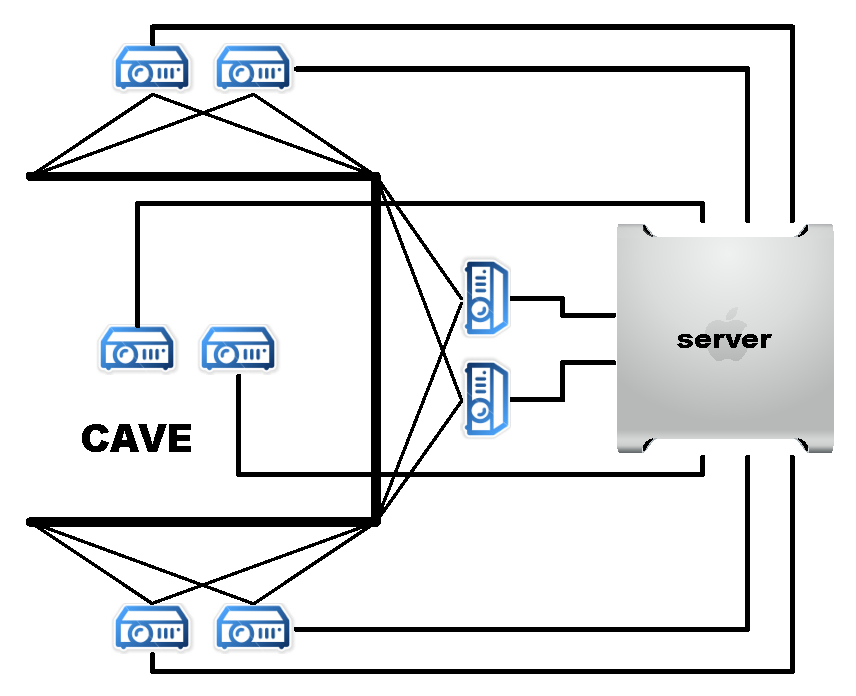
\includegraphics[width=0.8\textwidth]{../figures/1node_architecture}
	\caption{One-node setup}
	\end{figure}
\end{frame}

\subsubsection*{Six-node setup}
\begin{frame}\frametitle{Six-node setup}
	\begin{figure}
		\centering
	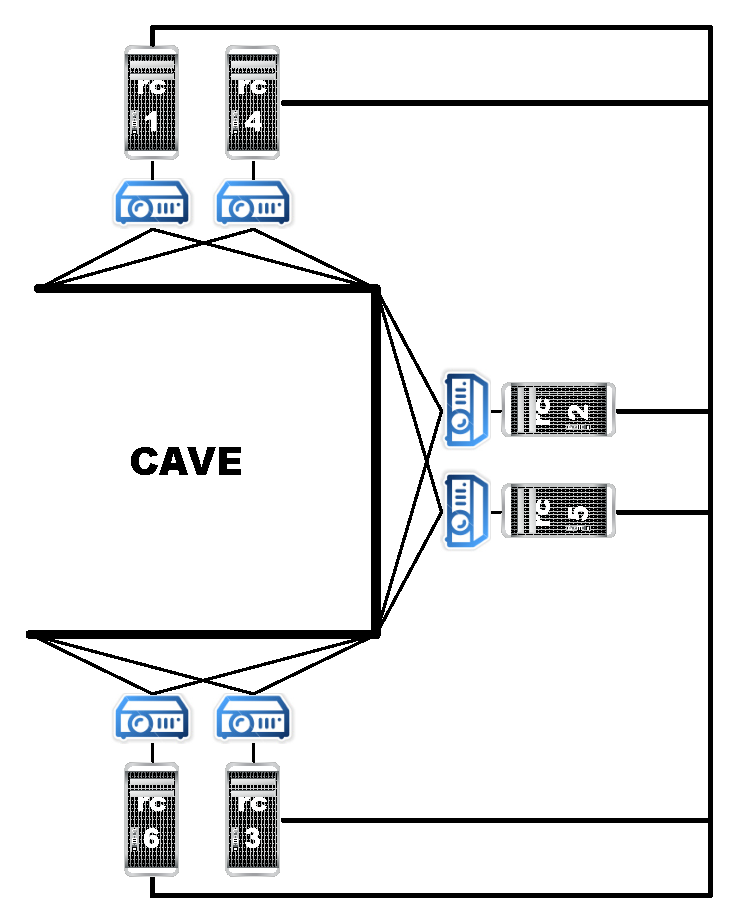
\includegraphics[width=0.6\textwidth]{../figures/6node_architecture}
	\caption{Network setup (6 nodes)}
	\end{figure}
\end{frame}

\subsection{Equalizer}
\begin{frame}\frametitle{Equalizer configuration files}
\begin{itemize}
	\item<1->One-node configuration
	\begin{itemize}
		\item Same physical workstation for server, application \& render clients
		\item Starting Equalizer server (\texttt{eqServer})
		\item Starting CRF application
	\end{itemize}
	\item<2->Six-node configuration
	\begin{itemize}
		\item 6 nodes connected via SSH
		\item 1 node acts as server
		\item Application \& data on each node
		\item Starting Equalizer server (\texttt{eqServer})
		\item Starting CRF application on server node $\rightarrow$ server starts application on all connected nodes
	\end{itemize}
\end{itemize}
\end{frame}

\subsubsection*{Notation}
\begin{frame}\frametitle{Equalizer configuration}
	\begin{description}
		\item[config] Configuration for a server
		\item[node] Abstraction of a workstation
		\item[connection] Point-to-point connection between nodes
		\item[pipe] Abstraction of a graphics card
		\item[window] Abstraction of a OpenGL drawable
		\item[channel] Viewport within a \emph{window}
		\item[compound] An ordered collection of tasks for a channel. Can have compound children.
	\end{description}
\end{frame}

\subsubsection*{One-node configuration}
\begin{frame}\frametitle{Equalizer one-node configuration}
	\begin{figure}
		\centering
		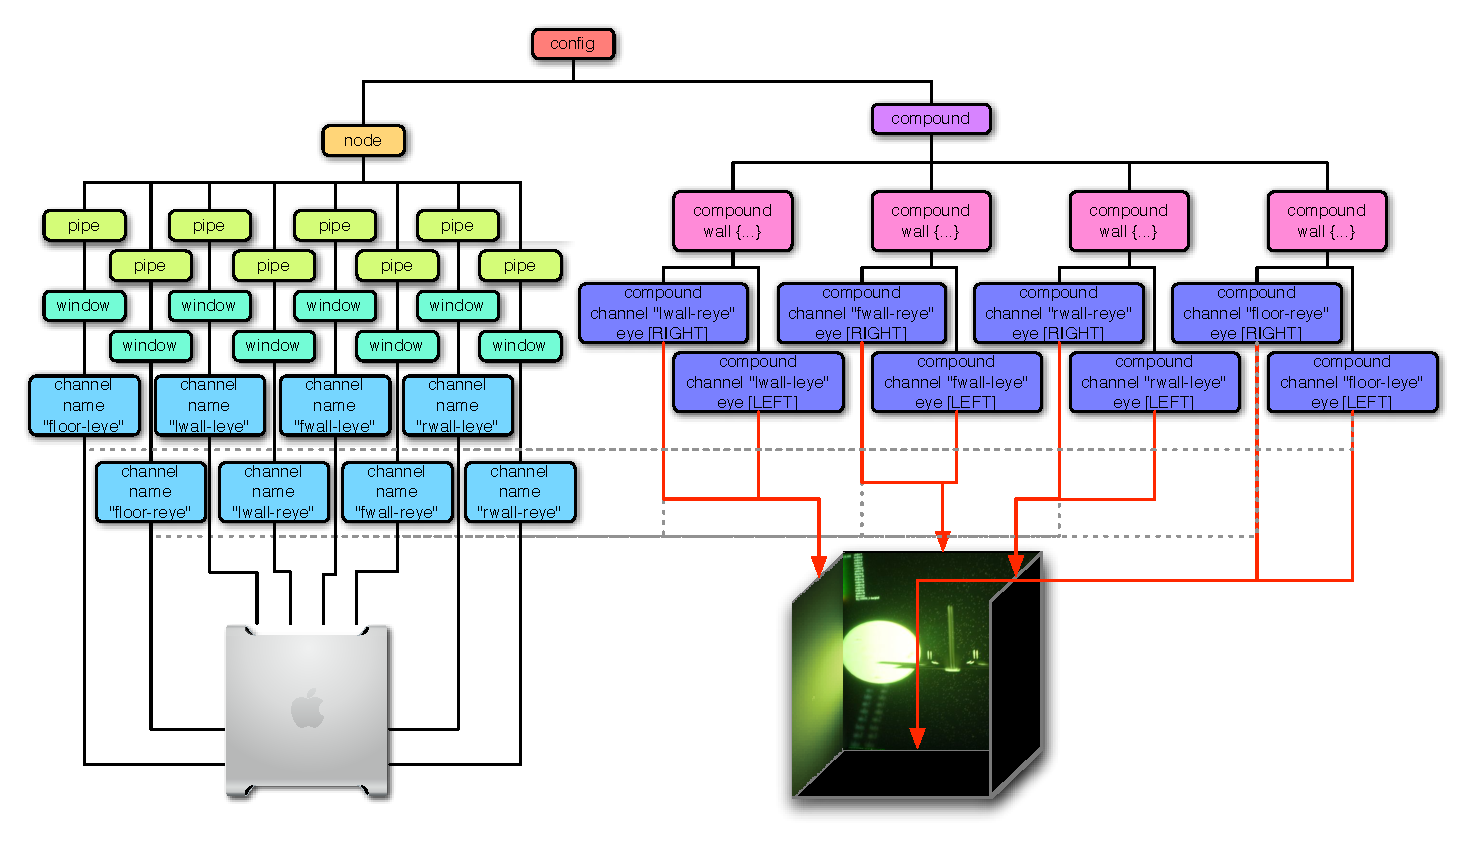
\includegraphics[width=\textwidth]{../figures/1nodeConfig}
		\caption{One-node Equalizer configuration}
	\end{figure}
\end{frame}

\subsubsection*{Six-node configuration}
\begin{frame}\frametitle{Equalizer six-node configuration}
	\begin{figure}
		\centering
		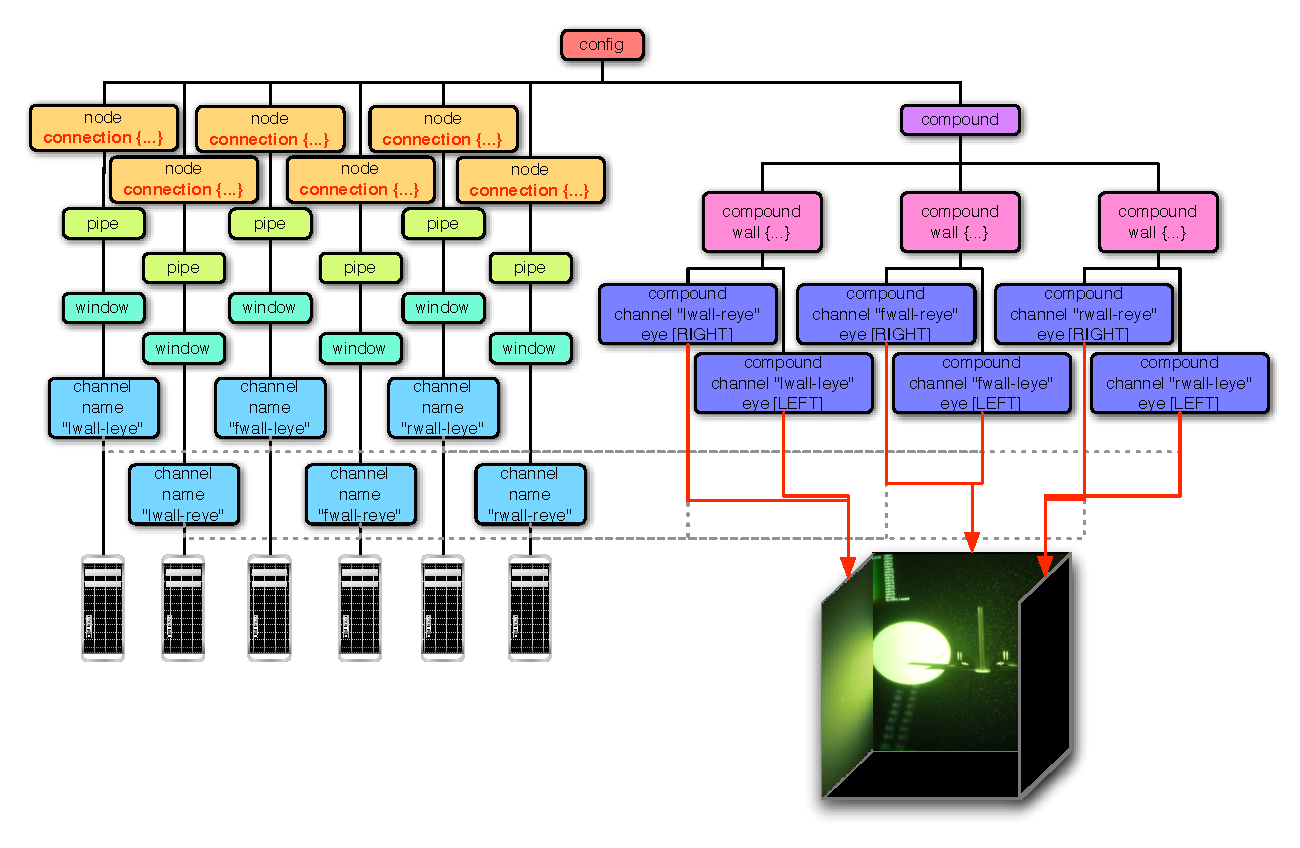
\includegraphics[width=\textwidth]{../figures/6nodeConfig}
		\caption{Six-node Equalizer configuration}
	\end{figure}
\end{frame}

\begin{frame}\frametitle{Equalizer conclusion}
	\begin{itemize}
		\item [+/-] Work in progress
		\item [+] Configurability
		\item [+] Active community
		\item [-] Combination of different hardware architectures may be a problem (32/64-bit)
		\item [-] High maintenance for network distributed solutions
	\end{itemize}
\end{frame}

\subsection{Framework}
\begin{frame}\frametitle{Framework - overview}
	\begin{itemize}
		\item<1-> Synchronisation
		\item<2-> Event handling
		\item<3-> Use of framework
		\item<4-> Conclusion
	\end{itemize}
\end{frame}

\subsubsection*{Synchronisation}
\begin{frame}\frametitle{Synchronisation}
	\begin{itemize}
		\item<1-> One OSG viewer per Equalizer pipe
		\item<2-> Each of these viewers holds a complete scene graph
		\item<3-> Synchronisation has to be respected
		\begin{itemize}
			\item Frame based animations
			\item Time based animations
			\item Event based animations
		\end{itemize}
	\end{itemize}
\end{frame}

\subsubsection*{Event handling}
\begin{frame}\frametitle{Event handling}
	\begin{itemize}
		\item<1-> Equalizer event handling
		\begin{itemize}
			\item Camera handling
			\item Statistics
		\end{itemize}
		\item<2-> Event propagation
		\begin{itemize}
			\item Selected Equalizer events are distributed
			\item Currently: Mouse- and most keyboard events
			\item Converted on every Equalizer pipe
		\end{itemize}
		\item<3-> OSG event handler
		\begin{itemize}
			\item OSG viewer(s) receive native OSG events
			\item Thus, common OSG event handlers can be used
		\end{itemize}
	\end{itemize}
	
\end{frame}

\subsubsection*{Use of framework}
\begin{frame}\frametitle{Use of framework}
	\begin{itemize}
		\item<1-> Abstraction
		\begin{itemize}
			\item Just basic Equalizer skills needed
			\item OSG applications can be easily ported to the CRF
			\item Just a few limitations
		\end{itemize}
		\item<2-> Facade pattern
		\begin{itemize}
			\item Hides the Equalizer initialisation from the CRF user
			\item Only two lines of code needed for a basic example
		\end{itemize}
		\item<3-> Overriding framework functions
		\begin{itemize}
			\item For more complex applications
			\item Well documented with examples
			\item Unlimited possibilities for further framework extensions
		\end{itemize}
	\end{itemize}
	
\end{frame}

\subsubsection*{Framework conclusion}
\begin{frame}\frametitle{Framework conclusion}
	\begin{itemize}
		\item<1-> Testing!
		\begin{itemize}
			\item Testing in real environments
			\item C++ is not easy!
			\item Multithreading can cause unexpected behaviours or even errors
			\item Black box tests for more improvements
		\end{itemize}
		\item<2-> Extensibility
		\begin{itemize}
			\item Numerous new features possible
			\item This is just a basic solution
		\end{itemize}
	\end{itemize}
\end{frame}
